\subsection{Independent measured sensor transfer}
\label{sec:pamap2}

Two co-located accelerometers in each PAMAP2 inertial unit measure
the same activity with different nominal ranges \cite{pamap2}.
We used the $\pm6g$ channels as inputs and the synchronized $\pm16g$
channels as measured references at the hand, chest and ankle.
The protocol was fixed locally before evaluating methods. It uses
6,660 disjoint windows of 200 samples from the official sessions of
eight participants. We omitted the participant with an incomplete
activity protocol. Each window contains one labeled activity and no
time gap above 0.025 seconds. The mean, standard deviation, RMS,
maximum absolute value and mean absolute increment for each axis give
45 features. These are paired hardware measurements without injected noise.

In each leave-one-subject-out fold we standardize by the training
reference and fit a multinomial logistic activity head on those
reference features. We freeze the head and preserve its decision on
the low-range input. A second consumer estimates the window's maximum
absolute acceleration across the recorded axes. We measure feature
MSE in the standardized space and peak MAE in $\mathrm{m/s^2}$,
averaging equally over participants. The predeclared near-range cohort
requires the observed peak to reach 95\% of the nominal $6g$ range.
It contains 604 windows. The reference reaches 95\% of its nominal
range in 47 windows, including 46 in the near-range cohort. It is
a measured reference channel with its own errors.

The fitted estimates include a mean offset, paired ridge calibration,
paired ExtraTrees calibration, and the Gaussian posterior mean and
flow. The paired calibrators predict the reference-minus-observed
residual from observed training features. All estimates can be used
directly, clipped or projected. The deployed segment for each
constrained estimate passes the same outward test in
Section~\ref{sec:reserve-verification}, at reserve $10^{-4}$ of the
original margins. An unverified candidate reverts to the input.
We independently certify the original flow at the largest accepted
fraction from $1,1/2,1/4,1/8$ of its intended horizon. The numerical
RK4 output must also pass the straight-segment check.

\begin{table}[htbp]
\centering
\small
\caption{PAMAP2 reference error on held-out subjects. Peak MAE is in
$\mathrm{m/s^2}$. The last column counts changed decisions across all
6,660 windows. Complete rows and subject results are archived.}
\label{tab:pamap2}
\begin{tabular}{lrrrrr}
\toprule
 & \multicolumn{2}{c}{Feature MSE} & \multicolumn{2}{c}{Peak MAE} & Changed \\
Method & All & Near range & All & Near range & (all) \\
\midrule
Observed input                  & .04408 & .33321 & 4.37 & 32.50 & 0 \\
Mean offset, projected          & .03516 & .29612 & 4.96 & 30.59 & 0 \\
Ridge                           & .02056 & .14982 & 3.54 & 18.81 & 386 \\
Ridge, clipped                  & .02061 & .14988 & 3.51 & 18.74 & 0 \\
Ridge, projected                & .02056 & .14981 & 3.54 & 18.80 & 0 \\
ExtraTrees                      & .02011 & .16938 & 2.79 & 19.28 & 330 \\
ExtraTrees, clipped             & .02025 & .16918 & 2.80 & 19.21 & 0 \\
ExtraTrees, projected           & .02011 & .16938 & 2.79 & 19.27 & 0 \\
Prototype mean, projected       & .04918 & .35833 & 4.62 & 33.10 & 0 \\
Local guarded flow              & .04824 & .35641 & 4.58 & 33.03 & 0 \\
\bottomrule
\end{tabular}
\end{table}

Projected ExtraTrees reduced the subject-average feature MSE
by 54.4\% relative to the observed input. The paired difference was
$-0.02397$ (descriptive subject-block bootstrap percentiles from
$-0.03268$ to $-0.01613$). Its peak MAE fell 36.1\%. Near the nominal
limit, projected ridge reduced feature MSE by 55.0\% and peak MAE by
42.2\%. Projection and clipping both retained the decision on all
windows. Their restoration errors were close in this benchmark.
Raw ExtraTrees and ridge changed 330 and 386 decisions, respectively.
Raw ExtraTrees classified 5,507 windows correctly. Constrained
predictions kept all 5,480 original correct decisions.

\begin{figure}[htbp]
\centering
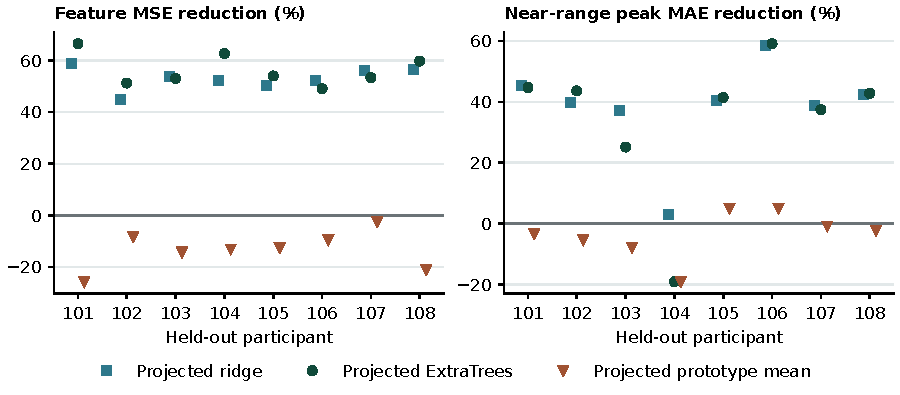
\includegraphics[width=\linewidth]{figures/pamap2_transfer.pdf}
\caption{Paired error reductions relative to the observed input for
each held-out participant. The same strict margin reserve applies to
all three projections. Positive values indicate lower reference error.}
\label{fig:pamap2-participants}
\end{figure}

The participant outcomes in Figure~\ref{fig:pamap2-participants} show
lower feature MSE for projected ExtraTrees in every fold and higher
MSE for the projected prototype estimate in every fold.

The local test certified the entire original flow horizon on 5,677
windows versus 3,017 for the global slab. The projected prototype mean
and guarded flow both increased feature error relative to the measured
input. The same verification procedure applies to estimates from better
fitted models. The outputs are feature vectors for downstream consumers.
A projected vector need not correspond to a physically realizable
acceleration time series. Fixed participants, overlapping training
folds and a single hardware source limit population inference.
